With our implementation done, it was time to benchmark our implementation on the cluster provided by the Department of Informatics (DI) of the NOVA University of Lisbon and evaluate the parallel performance by studying some performance metrics, such as speedup, efficiency and cost. 
\par In order to test and benchmark our solution, we implemented and used some python scripts for this effect:
\begin{itemize}
    \item \verb|TestsScriptBase.py| - is considered the base of the other scripts and contains all functions and variables necessary for the other scripts to run. The script has no effect by itself, and needs to be imported by the other scripts.
    \item \verb|Benchmark.py| - like the file name implies, is used to benchmark our solution. After the benchmark, the script will export the results metrics (mean time, speedup, efficiency, cost, etc...) to the \verb|seq.csv| and \verb|omp.csv| files, which contains the metrics about the sequential (\verb|energy_storms_seq|) and paralleled (\verb|energy_storms_omp|) programs samples metrics, respectively.
    \item \verb|RunCompare.py| - Used to test the paralleled version of the program with a specific number of threads by comparing the output with the original, sequential program. The script will run both programs once.
    \item \verb|TestFilesScript.py| - Tests all test files individually and combined (example: test all test\_02 files) in order to check the correctness of the paralleled program.     
    \item \verb|BuildPlot.py| - Produces a plot with the metrics about the \verb|Benchmark.py| results. The script imports the \verb|seq.csv| and \verb|omp.csv| files produced by the \verb|Benchmark.py| script and uses the Matplotlib python module to produce a plot.   
\end{itemize}
By default, the \verb|Benchmark.py| and \verb|TestFilesScript.py| scripts will execute the original program and the paralleled program for each number of threads 5 times (for example: the script will execute 5 times the program with 1 thread, 5 times with 2 threads, etc...).
\par We have to remark that the benchmarks on the cluster were done with the energy storms programs compiled with assertions disabled. Although assertions are a very handy tool to debug our program by testing our assumptions, they are not intended to be included on the production code, since it may cause side effects on the performance, depending on how they are implemented. 
\par Also, before doing the benchmark, we choose the adequate number of threads for the target node in the cluster given the number of cores, since executing the program with a number of threads above the available number of processing cores will not only not improve performance, but degrade it, as taught and shown in the practical classes of Concurrency and Parallelism.
\par Like mentioned before, in order to evaluate our solution after the benchmarks, it was used the following performance metrics, taught in the Concurrency and Parallelism classes:
\begin{itemize}
    \item \textbf{SpeedUp}
            \(S(p) = \frac{\texorpdfstring{T\textsubscript{1}}{nsub}}{T\textsubscript{p}}\)\\
    \item \textbf{Efficiency}
            \(E(p) = \frac{\texorpdfstring{S\textsubscript{p}}{nsub}}{p}\)\\
    \item \textbf{Cost}
            \(C(p) = p \times T\textsubscript{p}\)\\
\end{itemize}

Where \(T_{p}\) is the mean time of all program samples executed with \(p\) threads. Unfortunately, we detected near the deadline that the the efficiency plot on both \textbf{Figures 3 and 4} were generated from a previous version of the \verb|Benchmark.py| script that had a bug on the efficiency metric. This bug was fortunately corrected.

Originally, we expected that our energy bombardment optimization would improve considerably our program performance in comparison with the original, since we made the program "smart" by only updating the layer range above the threshold. However, as you can see in \textbf{Figure 3}, this expectation wasn't met with the default threshold value, given that it was so low that generally all energy increments caused by the particle collision on all layer positions were above the threshold. The small mean time gap between the original (\verb|SEQ| in the mean time plot) and the paralleled program with only one thread (\verb|OMP-1| in the mean time plot) is explained by the removal of the \verb|layer_copy| array, described in the energy relaxation phase section, which not only improved execution time by not initializing another array, but more obviously memory consumption, as we expected. 
\par In order to fully test our energy bombardment optimization, it was necessary to increase the program threshold value to a value that was enough to show notorious results. Looking at \textbf{Figure 3}, we see that the parallel program mean time was massively improved with a threshold value of 50. However, it is assumed that it was not the goal of the project to tune the threshold value, given that it was previously defined as a constant in the original program. But given that the threshold usually depends on the material of the layer, as mentioned in the project assignment, we though it was interesting to tune the threshold value with a program argument (-h).

\begin{figure}[h]
    \centering
    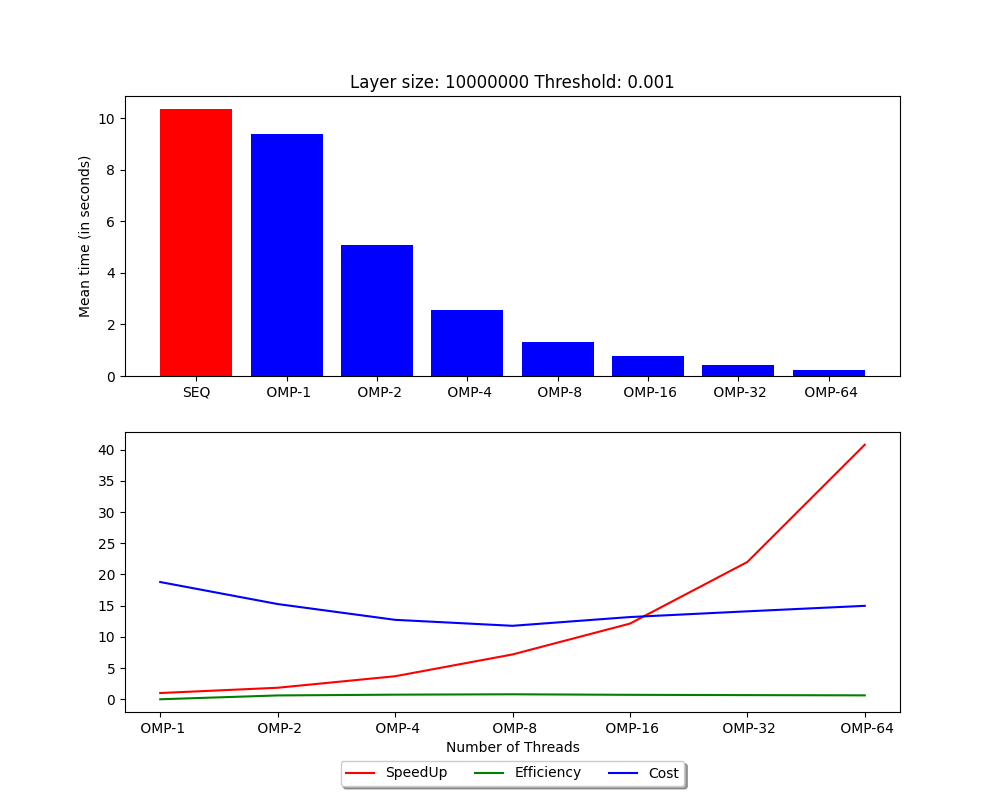
\includegraphics[scale=0.35]{images/plot_node12_all_test_01_ls_10000000.png}
    \caption{Using all test\_01 test files on node 12 with default threshold value}
    \label{fig:my_label}
\end{figure}
\begin{figure}[h]
    \centering
    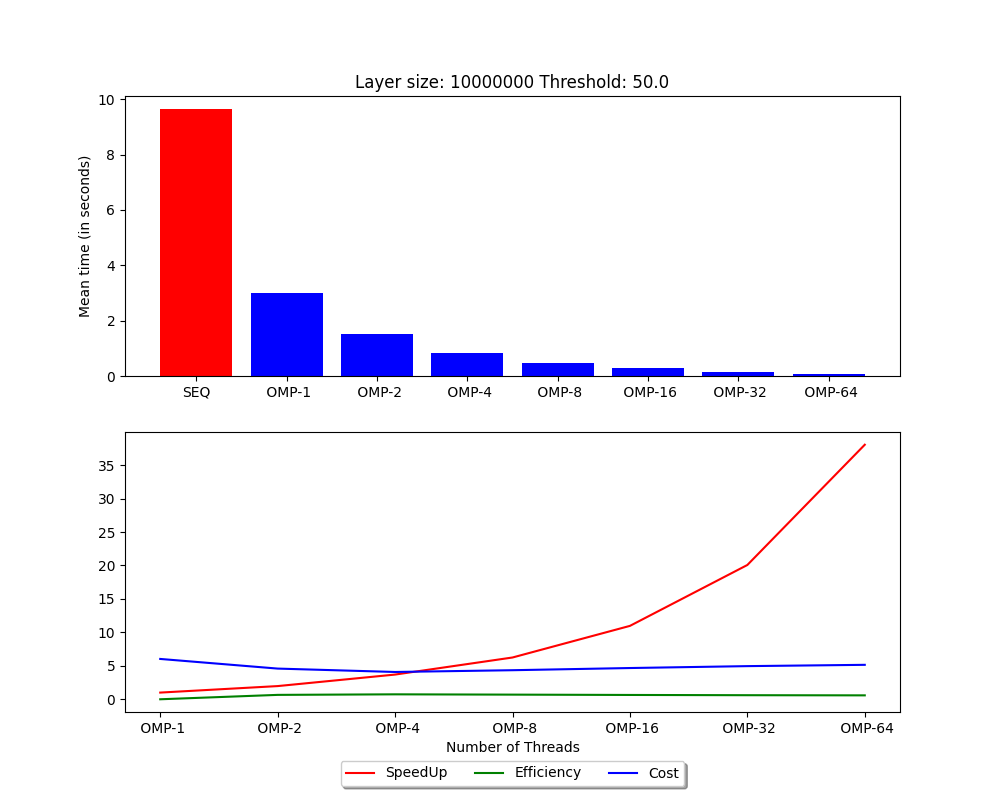
\includegraphics[scale=0.35]{images/plot_node12_all_test_01_ls_10000000_h_50.png}
    \caption{Using all test\_01 test files on node 12 with a threshold value of 50}
    \label{fig:my_label}
\end{figure}

When it comes to the parallelism metrics shown in the second plot of both figures, it is noted that the speedup on the paralleled program is exponentially increased as the number of threads increases, which implies that the meantime is decreasing, as shown in the first plot of both figures. This means that our program escalates well as the number of threads increases, which is a good thing and what we were expecting. However, evaluating program performance taking only into consideration speedup is not enough. Analyzing the cost metric, we can see that it is decreasing until 8 threads and increasing progressively after that. Besides that, although the efficiency plot values are too low and wrong, as stated before, we can compute the efficiency manually given the speedup, and we notice that it is progressively declining as the number of threads increases, which was expected.
